\chapter{Evaluación del sistema}
\label{cap:experimentos}

Con el sistema construido resta someterlo a evaluación. En especial se evalúa el sistema de detección de necesidades, pues es el corazón del sistema y ha de operar con un flujo de datos constante.

\section{Cumplimiento de requerimientos}
\label{seC:cumpRequerimientos}

En cuanto a la construcción del \textit{software}, se identificaron 12 historias de usuario y se especificaron cada uno de sus criterios de aceptación. Se pasa a detallar por cada historia si ésta fue cumplida o no.

\begin{itemize}
\item HU-c00: Mediante la construcción de un operador, \textit{Spout}, que haciendo uso del \textit{stream} de datos proporcionado por \textit{Twitter} recogiese los datos en tiempo real y la contrucción de un clasificador de texto es que se completó esta historia.
\item HU-c01: De igual manera que la historia anterior, haciendo uso de la información de \textit{Twitter}, esta historia se completó.
\item HU-c02: Esta historia se completó mediante la construcción del operador filtro de consulta, donde se añadió la capacidad de realizar \textit{query expansion}.
\item HU-v03: Se implementó mediante el actualizador del modelo de clasificación, dejando al usuario la tarea de etiquetar los datos para formar el conjunto de entrenamiento.
\item HU-c04: Se implementó mediante una base de datos no relacional en tres colecciones de datos: marcadores, \textit{tweets} y consultas.
\item HU-v00: Con la contrucción de la aplicación visualizadora, la que permite el despliegue de una interfaz \textit{Web} al usuario esta historia se marcó como completada.
\item HU-v01: Mediante el operador de ubicación esta historia de usuario se completó.
\item HU-v02: Se implementaron filtros haciendo uso de Javascript a la interfaz, permitiendo realizar veintidós formas de visualización diferentes.
\item HU-v03: Al igual que la historia anterior se utilizó Javascript, en específico AJAX, para que mediante un servicio REST se pudiese actualizar los nuevos marcadores.
\item HU-v04: Se utilizó una biblioteca externa, \textit{HighCharts}, para la implementación de una línea de tiempo con intervalo deslizante y mediante un servicio REST obtener los datos pertenecientes al intervalo seleccionado y cumplir así esta historia de usuario.
\item HU-v05: Se implementó junto con la historia de usuario HU-c02. El filtro de consultas permitía el paso de los \textit{tweets} que tuviesen parte de su contenido alguno de los términos especificados por el usuario.
\item HU-v06: Se diseñaron 7 iconos para corresponder a cada una de las categorías y completar esta historia, la descripción de estos es entregada por medio de la aplicación de visualización al usuario final.
\item HU-v07: Mediante la construcción de tres servicios REST que cuenten la cantidad de eventos desde la última consulta se completó esta historia de usuario.
\item HU-v08: Se permitió al usuario el parametrizar la configuración de la aplicación visualizadora, completando así esta historia de usuario.
\end{itemize}

\section{Evaluación del clasificador}
\label{sec:EvalClassificador}

En esta sección, el clasificador construido en la seción \ref{subsubsec:clasificacion} fue sometido a evaluación, se presentan en la Figura \ref{fig:metricasClass} los resultados correspondientes a las métricas obtenidas usando Mallet.

\begin{figure}[H]
        \centering
        \captionsetup{justification=centering}
        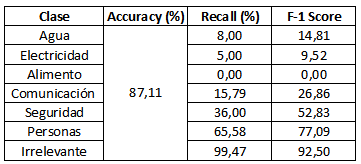
\includegraphics[scale=0.8]{images/MetricasClasificador.png}
        \caption[Métricas del clasificador.]{Métricas del clasificador.\\Fuente: Elaboración Propia, (2016)}
        \label{fig:metricasClass}
\end{figure}

Los valores expuestos anteriormente son interpretados, respectivamente, como sigue a continuación.

\begin{itemize}
\item \textit{Accuracy}: Este valor quiere decir qué con aproximadamente un 87\% al decir que un elemento pertenece a una determinada clase esa predicción es correcta.
\item \textit{Recall}: Este valor quiere decir que para una clase en particular es posible identificar en un determinado porcentaje $p$, correspondiente al valor presentado en la Figura \ref{fig:metricasClass}, de los elementos pertenecientes a aquella clase.
\item \textit{F-1 Score}: Corresponde al \textit{trade-off} entre \textit{accuracy} y \textit{recall}, al incrementar uno, el otro disminuye en un $F$\% descrito por los valores en la Figura \ref{fig:metricasClass}.
\end{itemize}

En particular este clasificador cuenta con alta precisión y bajo \textit{recall}, eso significa que es preciso para clasificar, pero es incapaz de clasificar algunos de los casos particulares de cada clase. Esto se debe al conjunto de entrenamiento utilizado, los datos no están balanceados para cada clase, es decir, la clase A no tiene la misma cantidad de datos utilizados para entrenar B. Esto repercute en que debido a las pocas instancias que tiene el algoritmo para aprender no es capaz de reconocer elementos de la clase con menos elementos. En particular el caso de la clase ``Alimentos", los datos que se utilizaron son del periodo inmediato al evento, por ello no se encontraron demasiados elementos que hagan referencia a la falta de alimento en una población. Específicamente, sólo se etiquetó un \textit{tweet} presentado en la Tabla \ref{tab:UnicoEstadoAlimento} dentro de la categoría alimento. Esto puede deberse a que el conjunto de \textit{tweets} utilizado corresponde a uno obtenido en el periodo inmediato del evento, probablemente si el conjunto contemplara \textit{tweets} obtenidos un tiempo después de la ocurrencia de éste, la cantidad de elementos clasificados dentro de la categoría alimentos aumentaría.

\begin{table}[H]
\centering
\captionsetup{justification=centering}
\caption[Estados dentro del conjunto de entrenamiento cuya categoría es alimento.]{Estados dentro del conjunto de entrenamiento cuya categoría es alimento.\\Fuente: Elaboracion Propia, (2016)}
\label{tab:UnicoEstadoAlimento}
\begin{tabular}{|c|l|}
\hline
\textbf{Categoría} & \multicolumn{1}{c|}{\textbf{Tweet}} \\ \hline
Alimento & \begin{tabular}[c]{@{}l@{}}"chilenos se vuelcan a supermercados y estaciones  \\ de servicio tras terremoto http://myloc.me/4giya"\end{tabular} \\ \hline
\end{tabular}
\end{table}

\section{Topología y replicación}
\label{sec:topYPar}

En la sección \ref{subsubsec:topologiaSistema} se explicitó cómo están dispuestos los operadores en la topología, pero se ha de recordar que el sistema está pensado para operar en casos de emergencia y ha de ser capaz de escalar de acuerdo a las necesidades de la situación.

\textit{Apache Storm} es capaz de realizar lo anterior, pero se ha de especificar el máximo número de nodos que tiene cada nivel de operadores. La Figura \ref{fig:Implementacion1} presenta la implementación de la topología inicial, mientras que la Figura \ref{fig:Implementacion1p2} presenta gráficamente cómo se vería esta topología.

\begin{figure}[H]
	\centering
	\captionsetup{justification=centering}
	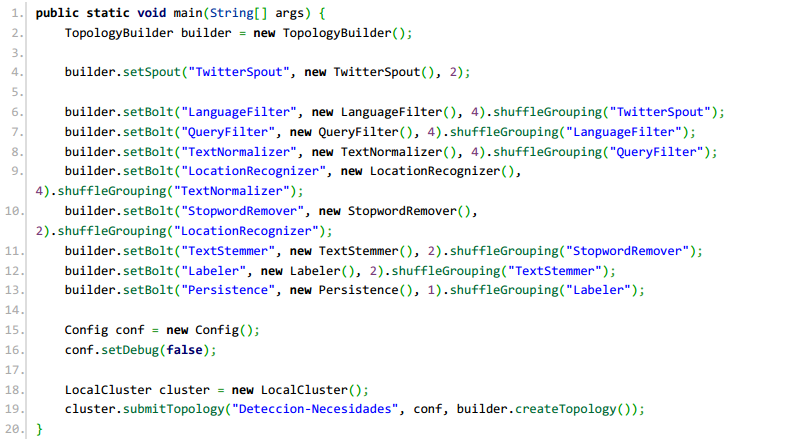
\includegraphics[scale=0.8]{images/ImplementacionTopologia1.png}
	\caption[Implementación topología de detección de necesidades.]{Implementación topología de detección de necesidades.\\Fuente: Elaboración Propia, (2016)}
	\label{fig:Implementacion1}
\end{figure}


La Figura \ref{fig:Implementacion1} se hace uso de una instancia de \textit{TopologyBuilder}, donde se especifican cada uno de los elementos de la topología. Para el caso de los \textit{Bolts} (líneas 6 a la 13), se hace uso del método \textit{setBolt}, al que además del nombre que tiene dentro de la topología, se entrega como parámetro una instancia del operador y se especifica cuál es su nivel de replicación. Además, se especifica el modo en el que se enviaran las tuplas para el procesamiento, en este caso, se hace uso de \textit{shuffle grouping} para entregarlas de forma \textit{round-robin} y balancear la carga en cada instancia del operador.

\begin{figure}[H]
	\centering
	\captionsetup{justification=centering}
	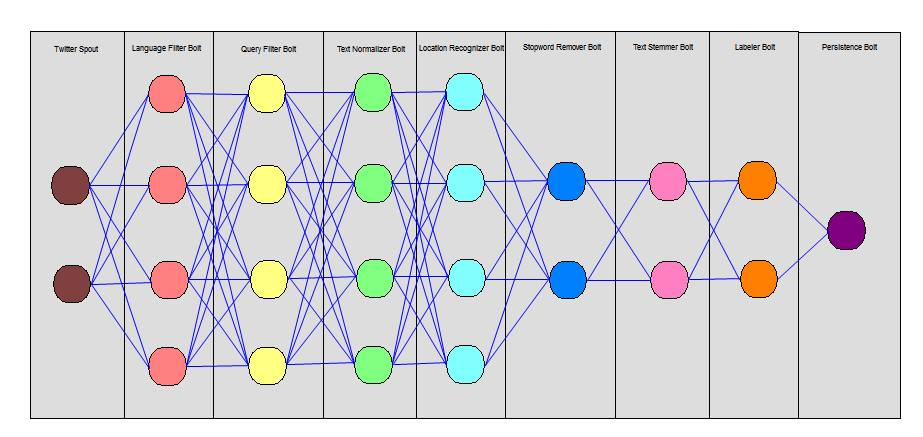
\includegraphics[scale=0.5]{images/ImplementacionTopologia1.2.png}
	\caption[Esquema de la topología en el caso de máxima actividad.]{Esquema de la topología en el caso de máxima actividad.\\Fuente: Elaboración Propia, (2016)}
	\label{fig:Implementacion1p2}
\end{figure}

Cada línea de este esquema presentado en la Figura \ref{fig:Implementacion1p2} señala comunicación de izquierda a derecha. En el caso de que el sistema trabaje al máximo de su capacidad cada nodo envía eventos al siguiente nivel usando el método round robin.

Al ejecutar la topología antes descrita se detectó que el hecho de tener dos \textit{spout} resultaba contraproducente, pues enviaba en repetidas ocasiones el mismo \textit{tweet} al sistema, es decir, cuando el \textit{spout} A enviaba el \textit{tweet}  $t_{0}$, probablemente el \textit{spout} B enviase el mismo \textit{tweet}  $t_{0}$, es decir, el resto del sistema procesaba el trabajo dos veces. Pora solucionar esto se decidió eliminar el segundo \textit{spout} y limitarlo sólo a uno.

Habiendo realizado lo anterior, se utilizó el tiempo de ejecución obtenido para el procesamiento de 1000, 2000, 4000 y 8000 eventos por esta topología, correspondientes a \textit{tweets} del terremoto de Concepción el año 2010 para seleccionar cuán numeroso debería ser un nivel de nodos. Sus resultados son expuestos en la Tabla \ref{tab:estadisticas}.

\begin{table}[H]
\centering
\caption[Estadísticas de los operadores diversos eventos.]{Estadísticas de los operadores diversos eventos.\\Fuente: Elaboración Propia, (2016)}
\label{tab:estadisticas}
\begin{tabular}{|c|c|c|c|c|c|}
\hline
\multirow{2}{*}{\textbf{\begin{tabular}[c]{@{}c@{}}Entradas \\ (eventos)\end{tabular}}} & \multirow{2}{*}{\textbf{Métricas}} & \multicolumn{4}{c|}{\textbf{Operadores}} \\ \cline{3-6} 
 &  & \textbf{Idioma} & \textbf{Normalizador} & \textbf{Ubicación} & \textbf{Stopword} \\ \hline
\multirow{4}{*}{\textbf{1000}} & \textbf{Procesados} & 1000 & 1000 & 1000 & 1000 \\ \cline{2-6} 
 & \textbf{Emitidos} & 402 (40.20\%) & 1000 (100\%) & 623 (62.30\%) & 1000 (100\%) \\ \cline{2-6} 
 & \textbf{Descartados} & 598 (59.80\%) & 0 (0\%) & 377 (37.70\%) & 0 (0\%) \\ \cline{2-6} 
 & \textbf{\begin{tabular}[c]{@{}c@{}}Tiempo \\ (ms)\end{tabular}} & 0.77 & 36,45 & 2111.73 & 30.54 \\ \hline
\multirow{4}{*}{\textbf{2000}} & \textbf{Procesados} & 2000 & 2000 & 2000 & 2000 \\ \cline{2-6} 
 & \textbf{Emitidos} & 807 (40.35\%) & 2000 (100\%) & 1058 (52.90\%) & 2000 (100\%) \\ \cline{2-6} 
 & \textbf{Descartados} & 1193 (59.65\%) & 0 (0\%) & 942 (47.10\%) & 0 (0\%) \\ \cline{2-6} 
 & \textbf{\begin{tabular}[c]{@{}c@{}}Tiempo\\ (ms)\end{tabular}} & 0.84 & 56.07 & 1314.53 & 45.23 \\ \hline
\multirow{4}{*}{\textbf{4000}} & \textbf{Procesados} & 4000 & 4000 & 4000 & 4000 \\ \cline{2-6} 
 & \textbf{Emitidos} & 1673 (41.83\%) & 4000 (100\%) & 1985 (49.63\%) & 4000 (100\%) \\ \cline{2-6} 
 & \textbf{Descartados} & 2327 (58.17\%) & 0 (0\%) & 2015 (50.37\%) & 0 (0\%) \\ \cline{2-6} 
 & \textbf{\begin{tabular}[c]{@{}c@{}}Tiempo\\ (ms)\end{tabular}} & 2.08 & 49.09 & 2155.30 & 71.09 \\ \hline
\multirow{4}{*}{\textbf{8000}} & \textbf{Procesados} & 8000 & 8000 & 8000 & 8000 \\ \cline{2-6} 
 & \textbf{Emitidos} & 3101 (38.76\%) & 8000 (100\%) & 4113 (51.41\%) & 8000 (100\%) \\ \cline{2-6} 
 & \textbf{Descartados} & 4899 (61.24\%) & 0 (\%) & 3887 (48.59\%) & 0 (0\%) \\ \cline{2-6} 
 & \textbf{\begin{tabular}[c]{@{}c@{}}Tiempo\\ (ms)\end{tabular}} & 3.37 & 59.53 & 4442.00 & 87.24 \\ \hline
\end{tabular}
\end{table}

Con estos resultados se busca definir el número de réplicas necesarias para cada operador a modo de reducir la latencia y mantener los datos fluyendo por cada nivel de \textit{bolts}. De los resultados presentados en la Tabla \ref{tab:estadisticas} se puede concluir lo siguiente:

\begin{enumerate}
\item Para el caso del operador filtro de idioma, para diferentes tamaños de conjuntos de estados, es emitido aproximadamente un 40.28\% del flujo de información que llega a aquel operador. Tiene un tiempo de ejecución reducido en comparación a los demás operadores.
\item En operadores normalizadores de texto y eliminación de \textit{stopwords} todo estado que llega es emitido.
\item El operador de ubicación admite, aproximadamente, un 54.06\% de los \textit{tweets} que llegan hasta él y presenta un elevado tiempo de ejecución.
\end{enumerate}

Estos resultados muestran el comportamiento individual de cada uno de estos \textit{bolts}, pero su operación no es de esta forma. Por ello se preparó el mismo conjunto de pruebas de 1000, 2000, 4000 y 8000 datos aleatorios del conjunto de datos del terremoto de Concepción el año 2010 y se pasó al sistema para ver la cantidad de eventos emitidos en cada caso. Para el caso del operador de consulta se utilizaron los términos ``terremoto", ``concepción" y ``Chile". Se restringió el paralelismo de la topología completa para realizar estas pruebas, es decir, cada operador tuvo como máximo una instancia trabajando durante todo el proceso.

\begin{table}[H]
\centering
\caption[Prueba sistema completo utilizando 1000 eventos.]{Prueba sistema completo utilizando 1000 eventos.\\Fuente: Elaboración Propia, (2016)}
\label{PruebaSistFull1000}
\begin{tabular}{|c|c|c|}
\hline
\textbf{Cantidad} & \multicolumn{2}{c|}{\textbf{1000}} \\ \hline
\textbf{Operador} & \multicolumn{1}{c|}{\textbf{Eventos recibidos}} & \multicolumn{1}{c|}{\textbf{Eventos emitidos}} \\ \hline
Spout & 1000 & 1000 \\ \hline
Idioma & 1000 & 402 \\ \hline
Consulta & 402 & 123 \\ \hline
Normalizador & 123 & 123 \\ \hline
Ubicacion & 123 & 0 \\ \hline
Stopword & 0 & 0 \\ \hline
Stemmer & 0 & 0 \\ \hline
Etiquetador & 0 & 0 \\ \hline
Persistencia & 0 & 0 \\ \hline
\end{tabular}
\end{table}

\begin{table}[H]
\centering
\caption[Prueba sistema completo utilizando 2000 eventos.]{Prueba sistema completo utilizando 2000 eventos.\\Fuente: Elaboración Propia, (2016)}
\label{PruebaSistFull2000}
\begin{tabular}{|c|c|c|}
\hline
\textbf{Cantidad} & \multicolumn{2}{c|}{\textbf{2000}} \\ \hline
\textbf{Operador} & \multicolumn{1}{c|}{\textbf{Eventos recibidos}} & \multicolumn{1}{c|}{\textbf{Eventos emitidos}} \\ \hline
Spout & 2000 & 2000 \\ \hline
Idioma & 2000 & 807 \\ \hline
Consulta & 807 & 78 \\ \hline
Normalizador & 78 & 78 \\ \hline
Ubicacion & 78 & 0 \\ \hline
Stopword & 0 & 0 \\ \hline
Stemmer & 0 & 0 \\ \hline
Etiquetador & 0 & 0 \\ \hline
Persistencia & 0 & 0 \\ \hline
\end{tabular}
\end{table}

\begin{table}[H]
\centering
\caption[Prueba sistema completo utilizando 4000 eventos.]{Prueba sistema completo utilizando 4000 eventos.\\Fuente: Elaboración Propia, (2016)}
\label{PruebaSistFull4000}
\begin{tabular}{|c|c|c|}
\hline
\textbf{Cantidad} & \multicolumn{2}{c|}{\textbf{4000}} \\ \hline
\textbf{Operador} & \multicolumn{1}{c|}{\textbf{Eventos recibidos}} & \multicolumn{1}{c|}{\textbf{Eventos emitidos}} \\ \hline
Spout & 4000 & 4000 \\ \hline
Idioma & 4000 & 1673 \\ \hline
Consulta & 1673 & 39 \\ \hline
Normalizador & 39 & 39 \\ \hline
Ubicacion & 39 & 0 \\ \hline
Stopword & 0 & 0 \\ \hline
Stemmer & 0 & 0 \\ \hline
Etiquetador & 0 & 0 \\ \hline
Persistencia & 0 & 0 \\ \hline
\end{tabular}
\end{table}

\begin{table}[H]
\centering
\caption[Prueba sistema completo utilizando 8000 eventos.]{Prueba sistema completo utilizando 8000 eventos.\\Fuente: Elaboración Propia, (2016)}
\label{PruebaSistFull8000}
\begin{tabular}{|c|c|c|}
\hline
\textbf{Cantidad} & \multicolumn{2}{c|}{\textbf{8000}} \\ \hline
\textbf{Operador} & \multicolumn{1}{c|}{\textbf{Eventos recibidos}} & \multicolumn{1}{c|}{\textbf{Eventos emitidos}} \\ \hline
Spout & 8000 & 8000 \\ \hline
Idioma & 8000 & 3101 \\ \hline
Consulta & 3101 & 151 \\ \hline
Normalizador & 151 & 151 \\ \hline
Ubicacion & 151 & 0 \\ \hline
Stopword & 0 & 0 \\ \hline
Stemmer & 0 & 0 \\ \hline
Etiquetador & 0 & 0 \\ \hline
Persistencia & 0 & 0 \\ \hline
\end{tabular}
\end{table}

Las Tablas \ref{PruebaSistFull1000}, \ref{PruebaSistFull2000}, \ref{PruebaSistFull4000} y \ref{PruebaSistFull8000} muestran respectivamente los resultados para los datos antes mencionados. Pueden ser leídas secuencialmente, es decir, presenta los estados que pasan por un operador y son entregados al siguiente. Estos resultados muestran la dificultad que tiene un \textit{tweet} para completar el proceso. Para confirmar que el sistema funcionase correctamente se incrementó la cantidad de datos, llegando a utilizar 30000 \textit{tweets} para evaluarlo. Los resultados se presentan en la Tabla \ref{tab:PruebaSistFull30000}.

\begin{table}[H]
\centering
\caption[Prueba sistema utilizando 30000 eventos.]{Prueba sistema utilizando 30000 eventos.\\Fuente: Elaboración Propia, (2016)}
\label{tab:PruebaSistFull30000}
\begin{tabular}{|c|c|c|}
\hline
\textbf{Cantidad} & \multicolumn{2}{c|}{\textbf{30000}} \\ \hline
\textbf{Operador} & \multicolumn{1}{c|}{\textbf{Eventos recibidos}} & \multicolumn{1}{c|}{\textbf{Eventos emitidos}} \\ \hline
Spout & 30000 & 30000 \\ \hline
Idioma & 30000 & 5372 \\ \hline
Consulta & 5372 & 883 \\ \hline
Normalizador & 883 & 883 \\ \hline
Ubicacion & 883 & 0 \\ \hline
Stopword & 0 & 0 \\ \hline
Stemmer & 0 & 0 \\ \hline
Etiquetador & 0 & 0 \\ \hline
Persistencia & 0 & 0 \\ \hline
\end{tabular}
\end{table}

Ninguno de los datos contenía información sobre la ubicación, por ello el operador encargado debe inferirla con respecto al texto, pero casos como el mostrado en la Tabla \ref{tab:resultadoEsperadoUbicacio} muestran que no se realizaba este proceso correctamente.

 \begin{table}[H]
\centering
\caption[Resultado esperado del operador de ubicación.]{Resultado esperado del operador de ubicación.\\Fuente: Elaboración Propia, (2016)}
\label{tab:resultadoEsperadoUbicacio}
\begin{tabular}{lllll}
\cline{1-3}
\multicolumn{1}{|c|}{\textbf{Eventos}} & \multicolumn{1}{c|}{\textbf{Resultado esperado}} & \multicolumn{1}{c|}{\textbf{Resultado obtenido}} &  &  \\ \cline{1-3}
\multicolumn{1}{|l|}{\begin{tabular}[c]{@{}l@{}}@tvn\_mauricio x fin internet desde el movil, \\ ciudad satelite maipu, sin luz ni agua desde \\ el terremoto casi 30 hrs\end{tabular}} & \multicolumn{1}{l|}{Emitir(-33.51667, -70.76667)} & \multicolumn{1}{l|}{No emitido} &  &  \\ \cline{1-3}
 &  &  &  &  \\
 &  &  &  & 
\end{tabular}
\end{table}

Habiendo realizado la corrección del proceso, se volvió a comprobar el comportamiento del sistema con el conjunto de 30000 \textit{tweets}. De esta comprobación se obtuvieron los resultados presentes en la Tabla \ref{tab:sistemaCompletoEstadosCorregidos}. Estos muestran que habiéndose producido el proceso de identificación, el último operador con las características de filtro, todos los estados pasaron a ser etiquetados y almacenados correctamente con la categorización realizada al ser evaluadas por el clasificador. 

Es importante volver a hacer hincapié en que si bien, estos u otros resultados se ven influenciados por los términos que compongan la consulta activa en un determinado momento, también la afectará el contexto de los \textit{tweets} recibidos hasta ese instante, pues con ellos se forma el conjunto de términos más usados, utilizado al expandir la consulta en este mismo operador.

\begin{table}[H]
\centering
\caption[Nueva prueba al sistema con 30000 eventos.]{Nueva prueba al sistema con 30000 eventos.\\Fuente: Elaboración Propia, (2016)}
\label{tab:sistemaCompletoEstadosCorregidos}
\begin{tabular}{|c|l|l|}
\hline
\textbf{Cantidad} & \multicolumn{2}{c|}{\textbf{30000}} \\ \hline
\textbf{Operador} & \multicolumn{1}{c|}{\textbf{Eventos recibidos}} & \multicolumn{1}{c|}{\textbf{Eventos emitidos}} \\ \hline
Spout & 30000 & 30000 \\ \hline
Idioma & 30000 & 5372 \\ \hline
Consulta & 5372 & 883 \\ \hline
Normalizador & 883 & 883 \\ \hline
Ubicacion & 883 & 743 \\ \hline
Stopword & 743 & 743 \\ \hline
Stemmer & 743 & 743 \\ \hline
Etiquetador & 743 & 743 \\ \hline
Persistencia & 743 & 743 \\ \hline
\end{tabular}
\end{table}

Estos resultados distan de los realizados para los operadores individuales y muestran que el flujo de información en el sistema haciendo uso de datos reales. Teniendo en cuenta estos resultados se modifica la topología inicial presentada en la Figura \ref{fig:Implementacion1p2} y pasa a utilizarse la presentada en la Tabla \ref{tab:topologiaFinal}. Sus valores se basan en el porcentaje de datos capaces de pasar el operador, siendo estos representados en la Tabla \ref{tab:topologiaFinal2}.

\begin{table}[H]
\caption[Nivel general de replicación de la topología.]{Nivel general de replicación de la topología.\\Fuente: Elaboración Propia, (2016)}
\centering
\label{tab:topologiaFinal2}
\begin{tabular}{|l|c|}
\hline
\multicolumn{1}{|c|}{\textbf{Operador}} & \textbf{Nivel de replicación} \\ \hline
Spout & 1 \\ \hline
Idioma & N \\ \hline
Consulta & C = $\ceil{18\% · N}$ \\ \hline
Normalizador & $\ceil{16\% · C}$ \\ \hline
Ubicación & U = $\ceil{16\% · C}$ \\ \hline
Stopword & S = $\ceil{84.14\% · U}$ \\ \hline
Stemmer & S \\ \hline
Etiquetador & S \\ \hline
Persistencia & S \\ \hline
\end{tabular}
\end{table}
        
En la Tabla \ref{tab:topologiaFinal2} es un valor arbitrario determinado por el desarrollador. Para determinar un nivel de replicación para el sistema se determinó $N = 10$, así el sistema se entrega como el siguiente nivel de replicación máximo en sus operadores:

\begin{table}[H]
\centering
\caption[Nivel máximo de replicación de la topología.]{Nivel máximo de replicación de la topología.\\Fuente: Elaboración Propia, (2016)}
\label{tab:topologiaFinal}
\begin{tabular}{|l|c|}
\hline
\multicolumn{1}{|c|}{\textbf{Operador}} & \textbf{Nivel de replicación} \\ \hline
Spout & 1 \\ \hline
Idioma & 10 \\ \hline
Consulta & 2 \\ \hline
Normalizador & 2 \\ \hline
Ubicación & 2 \\ \hline
Stopword & 1 \\ \hline
Stemmer & 1 \\ \hline
Etiquetador & 1 \\ \hline
Persistencia & 1 \\ \hline
\end{tabular}
\end{table} 

\section{Funcionamiento en alto tráfico}
\label{sec:AltoTrafico}

La siguiente gráfica presentada en la Figura \ref{fig:graficoDeTweets} presenta el flujo de mensajes de \textit{Twitter} entre las fechas 16 de febrero y 2 de marzo del año 2010 perteneciente al conjunto de datos utilizado, en ella se aprecia que se produjo un \textit{peak} de \textit{tweets} al momento de producirse el evento terremoto.

\begin{figure}[H]
        \centering
        \captionsetup{justification=centering}
        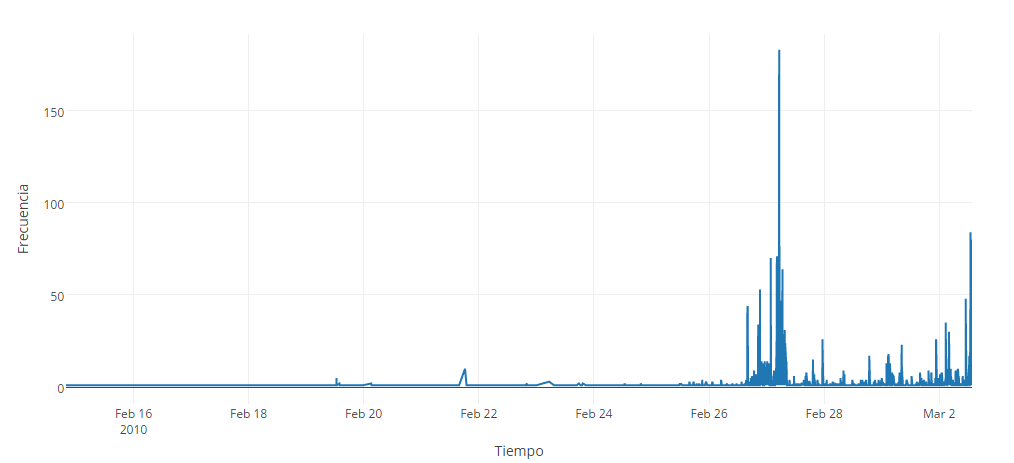
\includegraphics[scale=0.6]{images/GraficoTweetsHastaEventoZoom1.png}
        \caption[Distribución de eventos presente en el conjunto de datos utilizado para evaluar.]{Distribución de estados presente en el conjunto de datos utilizado para evaluar.\\Fuente: Elaboración Propia, (2016)}
        \label{fig:graficoDeTweets}
\end{figure}

Este \textit{peak} en la generación de datos no se ve reflejado como un aumento en la cantidad de datos que llegan al \textit{spout}, pues la cantidad de mensajes por segundo ingresados por \textit{Twitter4J} al sistema es constante mientras esté bajo la cuota límite de \textit{Twitter}. En el sistema este incremento se vería reflejado, probablemente, en un aumento de los \textit{tweets} que aprueben el filtro de consultas si se están utilizando términos relacionados a este evento.

Teniendo en consideración lo anterior en cuanto a la cantidad de mensajes, se realizó una recopilación de eventos por un periodo de una hora del \textit{stream} actual de eventos para obtener un total de 100.800 \textit{tweets}. El gráfico presente en la Figura \ref{fig:graficoAcumulado} muestra la cantidad eventos acumulados en función del tiempo cuya pendiente indica que se reciben 42 eventos por segundo en promedio.

\begin{figure}[H]
        \centering
        \captionsetup{justification=centering}
        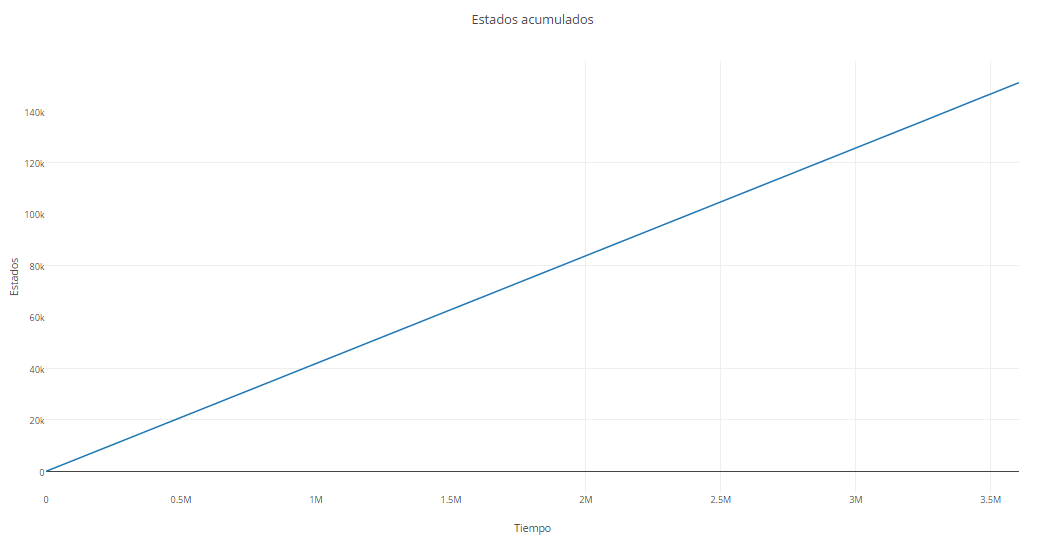
\includegraphics[scale=0.5]{images/DatosAcumulados.png}
        \caption[Recopilación de datos desde el \textit{stream}.]{Recopilación de datos desde el \textit{stream}.\\Fuente: Elaboración Propia, (2016)}
        \label{fig:graficoAcumulado}
\end{figure}

Haciendo uso de estos resultados se simuló la llegada de los eventos contenidos dentro de los datos de prueba sobre el sistema. Los resultados de esta simulación del comportamiento de la aplicación al operar como si fuese un evento real se muestran a continuación. La máquina para realizar estas pruebas fue la descrita en la sección \ref{subsec:HerrDesarrollo} y se utilizó la herramienta YourKit. Se utilizaron 100.000 \textit{tweets} del terremoto para realizar esta simulación y no se limitó la cantidad de eventos por segundo para probar el comportamiento del sistema con una carga de trabajo mayor a la habitual.

\begin{figure}[H]
        \centering
        \captionsetup{justification=centering}
        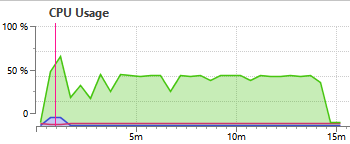
\includegraphics[scale=1.2]{images/CPUUsageN.png}
        \caption[Uso de CPU durante la simulación.]{Uso de CPU durante la simulación.\\Fuente: Elaboración Propia, (2016)}
        \label{fig:cpuUsage}
\end{figure}

La gráfica presentada en la Figura \ref{fig:cpuUsage} muestra el uso de la CPU del proceso \textit{DeNe-Core} durante la simulación realizada, se ve gran variación del uso de CPU al comienzo de la operación, esto se debe al uso de un \textit{Spout} alternativo encargado de emitir los \textit{tweets} almacenados en un archivo del tipo JSON correspondientes al evento del año 2010, esto se aprecia en la Figura \ref{fig:fileOpenClose} que muestra la cantidad de archivos abiertos en el tiempo. Posterior a la carga de los datos al sistema, sin considerar el primer segmento, el uso de CPU se mantiene constante alrededor del 49\% y permanece cercano a ese valor hasta que terminan de procesarse todos los \textit{tweets}, aproximadamente a 10 minutos desde el inicio de la prueba. Teniendo en consideración que se entregaron 100.000 \textit{tweets} se procesan alrededor de 166 por minuto en esta prueba, eso es aproximadamente un 400\% más de lo que es posible recoger desde el \textit{stream} de \textit{Twitter}, por lo que se espera que en condiciones normales de operación, y dada la limitante del tiempo real, el uso del CPU sea menor al presentado en esta prueba. Siempre teniendo en cuenta que la cantidad de mensajes que alcanzan la mayor parte del sistema están dados en función de los términos de búsqueda especificados por el usuario. Para este caso, se utilizaron los mismos términos especificados anteriormente: ``terremoto", ``Chile" y ``Concepción."

A pesar de que esta es una prueba a pequeña escala, ya ha sido validado por otros sistemas la capacidad de escalar de los sistemas de procesamiento como \textit{Storm}, ejemplo de ello son los trabajos realizados por \citep{WladdimiroElastic}, \citep{sclnStorm}, \citep{HowSpotifyScalesStorm}, entre otros.

\begin{figure}[H]
        \centering
        \captionsetup{justification=centering}
        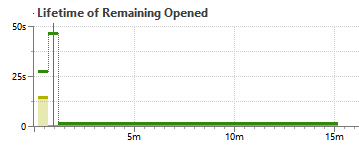
\includegraphics[scale=1.2]{images/FileOpenedClosed.png}
        \caption[Archivos abiertos durante la simulación.]{Archivos abiertos durante la simulación.\\Fuente: Elaboración Propia, (2016)}
        \label{fig:fileOpenClose}
\end{figure}

--- FALTA AGREGAR CONCLUSIÓN ---


